\subsection{Campo de aplicación}

\textbf{Contenedores de Basura Inteligentes}

Los contenedores de basura inteligentes encuentran aplicaciones en varios sectores:

\subsubsection{Entornos Urbanos}
En ciudades y municipios, los contenedores de basura inteligentes están ayudando a gestionar grandes volúmenes de residuos de manera eficiente. Son particularmente útiles en áreas de mucho tráfico, ya que reducen la carga de trabajo de los equipos de recolección de residuos \cite{buying}.

El Internet de las Cosas está teniendo un impacto tanto en la industria como en la vida cotidiana de las personas. Actualmente existen contenedores de basura inteligentes, que han funcionado exitosamente en ciudades como Sevilla. A través del proyecto europeo LIFE EWAS, se ha implementado una solución de TICS que permite monitorizar el volumen de llenado de los contenedores. Se implementan sensores con sistemas de medidas volumétricas basados en parámetros como la distancia, es decir, el trecho entre el nivel de residuos y el sensor. Esta información permite conocer la capacidad de un contenedor. Al dotar de inteligencia al contenedor, se puede entregar información a un gestor de servicios, optimizando así la recolección de los residuos \cite{quimbita}.

\begin{figure}[htb]
	\centering
	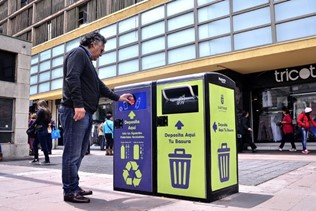
\includegraphics[scale  = 0.90]{Imagenes/basurero int.jpg}
	\caption{Basurero inteligente}{Fuente: Adaptado de~\cite{chile}}

\end{figure}

\subsubsection{Espacios Comerciales}
En entornos comerciales, como centros comerciales y aeropuertos, los contenedores inteligentes mejoran la gestión de residuos, asegurando que se vacíen rápidamente y reduciendo las molestias del desbordamiento de basura \cite{buying}.

\subsubsection{Industria Hotelera}
Los hoteles y restaurantes están utilizando contenedores inteligentes para mantener la limpieza y la higiene, brindando una mejor experiencia a los huéspedes \cite{buying}. Los botes de basura inteligentes pueden mejorar la experiencia del cliente proporcionando una gestión automática y sin contacto, aumentando la comodidad y reduciendo la necesidad de mantenimiento frecuente. Pueden notificar cuando están llenos, asegurando que el personal de limpieza los vacíe de manera oportuna, lo cual es una buena manera de asegurar que los clientes no se disgusten y se sientan bien atendidos.

\subsubsection{Instalaciones Sanitarias}
En entornos sanitarios, donde la higiene es primordial, los contenedores de basura inteligentes desempeñan un papel crucial en la gestión eficiente de residuos y el control de infecciones \cite{buying}.

\subsubsection{Instituciones Educativas}
Las escuelas y universidades están utilizando contenedores inteligentes para enseñar a los estudiantes sobre la eliminación responsable de residuos y, al mismo tiempo, mantener limpios sus campus. Este es uno de los campos de aplicación que motivan este proyecto, ya que son situaciones comunes en las instituciones educativas en el día a día.
